\chapter{Anwendung von LLM Tools im Software Engineering} \index{Anwendung von LLM Tools im Software Engineering}

\begin{figure}
    \centering
    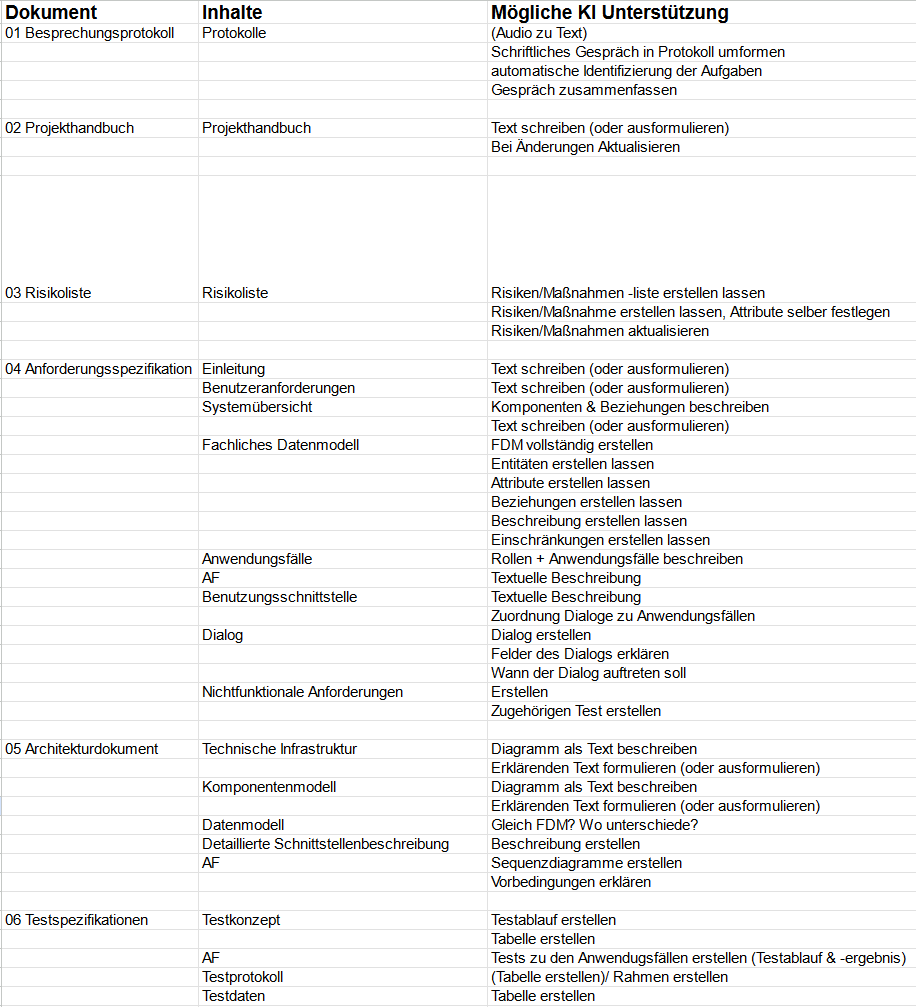
\includegraphics{pictures/Kapitel3Tabelle.PNG}
    \caption{Mögliche LLM Tool Unterstützung}
    \label{Dokumente mit LLM}
\end{figure}

Dieses Kapitel benennt einige potenzielle Anwendungsfälle von LLM-Tools in der Erstellung der Dokumente aus dem 
Software Engineering Prozess und anschließend wird festgelegt, was im folgenden Kapitel der Arbeit, der Analyse 
der Ausgaben der Tools, versucht wird zu erstellen. Die \autoref{Dokumente mit LLM} bietet eine Übersicht 
darüber, in welchen Dokumenten und bei welchen Inhalten LLM-Tools unterstützend eingesetzt 
werden können und dient als Beschreibung der Aufgabe für das nächste Kapitel.

\section{Besprechungsprotokoll} \index{Besprechungsprotokoll} \label{LLMBesprechungsprotokoll}

Im \autoref{Besprechungsprotokoll} wurde bereits erläutert, welche Inhalte in einem Besprechungsprotokoll enthalten 
sind. Nun stellt sich die Frage, wie LLM-Tools bei der Erstellung eines solchen Dokuments unterstützen können.

Eine Möglichkeit wäre, das Besprechungsprotokoll aufzeichnen zu lassen und anschließend automatisch daraus das Protokoll 
erstellen zu lassen. Da aktuell jedoch nur die kostenfreie Version ChatGPT-4o mit Dokumenten arbeiten kann, ist dies 
nur in begrenztem Umfang und ohne Vergleiche testbar, weshalb dies hier nicht betrachtet wird.

Daher wäre eine Möglichkeit, das Meeting zu verschriftlichen und damit als Texteingabe zu arbeiten. Mit dem 
schriftlichen Gespräch könnten die Tools dann automatisch die Tabelle des Besprechungsprotokoll erstellt 
werden. Die beim Besprechungsprotokoll zu beginn aufgezählten Daten  Datum, Thema, Verfasser, Teilnehmer 
und Verteiler könnten dabei 
vernachlässigt werden, da diese Informationen vermutlich extra in die Eingabe eingefügt werden müssten damit 
diese erstellt werden würden. Dadurch gäbe es kein Zeitersparnis oder sonstigen Vorteil, sich dies erstellen 
zu lassen.


\section{Projekthandbuch} \index{Projekthandbuch} \label{LLMProjekthandbuch}

Das Projekthandbuch ist ein zentrales Dokument im Software Engineering Prozess, das alle wesentlichen Informationen und 
Richtlinien eines Projekts zusammenfasst. Die spezifischen Inhalte dieses Dokuments wurden bereits im 
\autoref{Projekthandbuch} dargelegt. Doch wie können LLM-Tools bei der Erstellung des 
Projekthandbuches unterstützend wirken?

Hier wird sich auf die Abschnitte ``Zweck des Dokuments'', ``Redaktion'' und ``Verteiler'' im Kapitel ``Einleitung''
und auf die Abschnitte ``Vorgeschichte'' und ``Inhaltliche Kurzdarstellung'' im Kapitel ``Projektdefinition'' beschränkt. 
Dies hat den Grund, dass sich die restlichen Abschnitte des Projekthandbuches aus den Unterlagen für das Modul ``Secure Software 
Engineering'' ergeben und hauptsächlich als Bild aus der Präsentation in das Projekthandbuch eingefügt werden.\\
Die aufgezählten Abschnitte könnte man versuchen, sich automatisch erstellen zu lassen. Falls spezifische Informationen 
dafür benötigt werden, müssten diese mit in die Eingabe geschrieben werden.

\section{Risikoliste} \index{Risikoliste} \label{LLMRisikoliste}

Nachdem im \autoref{Risikoliste} die Bestandteile der Risikoliste beschrieben wurden, stellt sich auch hier die Frage, 
wie LLM Tools bei der Erstellung und Pflege der Risikoliste mitwirken und unterstützen können.

Eine Möglichkeit besteht darin, die gesamte Risikoliste einschließlich der zugehörigen Maßnahmentabelle von 
LLM Tools erstellen zu lassen. Dabei sollten alle Attribute für die Risiken festgelegt werden. Die Werte der einzelnen 
Risikoattribute sollten zudem zueinander in einem konsistenten Verhältnis stehen.


\section{Anforderungsspezifikation} \index{Anforderungsspezifikation} \label{LLMAnforderungsspezifikation}

Das \autoref{Anforderungsspezifikation} beschreibt die einzelnen Inhalte der Anforderungsspezifikation. Doch wie 
können LLM-Tools bei der Erstellung dieser unterstützen?

Zunächst könnte die Einleitung des Dokuments komplett von den Tools erstellt werden. Falls hier spezifische 
Informationen benötigt werden, sollten diese mit in die Eingabe eingefügt werden.

Danach kommt die Systemübersicht. Da außer ChatGPT-4o keines der Tools eigenständig Dokumente erstellen kann, 
wird die Zeichnung vermutlich selbstständig erstellt werden müssen. Es sollte jedoch möglich sein, die 
Beschreibung der Komponenten und deren 
Beziehungen von den Tools erstellen zu lassen und diese Beschreibung dann selbstständig in eine Zeichnung 
umzusetzen. Ebenso 
kann der Text, der das System beschreibt und in die Systemlandschaft einordnet, automatisch generiert werden. Der 
Fokus liegt hier allerdings auf der Zeichnung bzw. auf der Beschreibung der Komponenten und deren Beziehungen.

Ähnlich verhält es sich beim fachlichen Datenmodell. Hier könnte das UML-Klassendiagramm als 
PlantUML-Code oder einen ähnlichen Code ausgegeben werden. Da dies dann allerdings eher an den Programmierfähigkeiten 
scheitert als an der Fähigkeit, ein fachliches Datenmodell zu erstellen, ist dies keine Bedingung, die mit in die Bewertung 
einfließt, sondern ein nettes extra wäre. Die Beschreibung des Diagramms sollte dann allerdings so gut sein, dass die Erstellung 
manuell erfolgen kann. Die dazugehörigen Beschreibungen und Einschränkungen können ebenfalls von den Tools generiert werden.

Anschließend folgt das Anwendungsfalldiagramm. Dieses könnte ebenfalls mittels PlantUML oder ähnlichen Tools grafisch 
erstellt werden, was aber auch hier, aus oben angegebenen Gründen keine Bedingung ist. Andernfalls können 
die LLM-Tools die Rollen, deren Verbindungen und die zugehörigen Anwendungsfälle auflisten. Falls zusätzliche 
Bemerkungen zu den Anwendungsfällen erforderlich sind, können diese auch von den Tools erstellt werden.

Bei den detaillierten Beschreibungen der einzelnen Anwendungsfälle mit Aktivitätsdiagramm sollte der Fokus auf 
dem Aktivitätsdiagramm und den dazugehörigen Beschreibungen der Aktivitäten liegen. Das Aktivitätsdiagramm 
könnte ebenfalls mit PlantUML oder ähnlichen Tools erstellt werden. Dies ist aber auch hier keine Anforderung an 
die Tools wegen den oben angegebenen Gründen. Falls dies jedoch nicht erstellt werden kann, ist eine genaue 
und detaillierte Beschreibung des Aktivitätsdiagramms erforderlich. Die Beschreibung der Aktivitäten 
sollte, unabhängig von der Darstellung des Diagramms, vollständig von den Tools generiert werden können.

Darauf folgt die Benutzungsschnittstelle welche entweder vollständig durch PlantUML-Code oder ähnlichen Tools 
oder textuell beschrieben werden sollte. Die zusätzliche Bemerkungen und die Zuordnung der Dialoge zu den Anwendungsfällen 
spielen hier erst einmal eine untergeordnete Rolle.

Die einzelnen Dialoge können textuell beschrieben werden oder in den Chat ``skizziert'' werden, wobei es egal ist, 
für was sich die Tools entscheiden. Die einzelnen Eingabefelder und Buttons sollten ebenfalls erläutert werden sowie 
die Beschreibung, wann der Dialog aufgerufen wird und was beim Schließen des Dialogs passiert, sollten erstellt werden.

Zuletzt werden die nichtfunktionalen Anforderungen mitsamt den dazugehörigen Tests aufgelistet. Beides sollte 
von Tools eigenständig erstellt werden können.

\section{Architekturdokument} \index{Architekturdokument} \label{LLMArchitekturdokument}

Das Architekturdokument beschreibt die grundlegende Struktur und die Designentscheidungen eines Softwareprojekts. 
Die genauen Inhalte wurden bereits im \autoref{Architekturdokument} erläutert. Doch wie können LLM-Tools bei der 
Erstellung dieses Dokuments unterstützen?

Die technische Infrastruktur besteht aus einer Grafik und einem erklärenden Text. Die Erstellung der Grafik 
könnte wieder als ``Skizze'' im Chat erstellt werden, was aber keine Anforderung an die Tools ist. Wenn 
eine Skizze erstellt wird, sollte aber ein erklärender Text mit erstellt werden. Ansonsten wird sich auf 
die Erstellung der Grafik konzentriert. Ob dies dabei in Stichpunkten oder als Fließtext erfolgt, ist dabei 
zunächst egal.

Anschließend folgt das Komponentenmodell. Dieses könnte wieder in PlantUML oder ähnlichen Tools erstellt 
werden. Es kann auch eine detaillierte Beschreibung erstellt werden. Hierzu gibt es einen begleitenden Text, der die 
Komponenten und Schnittstellen beschreibt und deren Funktion erläutert. Ob dies in Stichpunkten oder als 
Fließtext erstellt wird spielt auch hier keine Rolle. Ausschlaggebend und das Hauptaugenmerk liegt auf dem 
Komponentenmodell.

Nach der Schnittstellenbeschreibung folgt die dynamische Beschreibung exemplarischer Anwendungsfälle. Diese besteht 
aus einem Sequenzdiagramm und den für den Anwendungsfall benötigten Vorbedingungen. Das Sequenzdiagramm kann ebenfalls 
als PlantUML-Code oder ähnlich erstellt werden, was aber keine Anforderung an die Tools ist. Falls dies nicht klappt 
reicht auch eine detaillierte Beschreibung des Diagramms. Die Vorbedingungen sollten ohne Schwierigkeiten 
generiert werden können, spielt hier aber zunächst keine Rolle. Das Hauptaugenmerk liegt wieder auf dem Diagramm.

\section{Testspezifikation} \index{Testspezifikation} \label{LLMTestspezifikation}

Im \autoref{Testspezifikation} wurde bereits erklärt, welche Inhalte die Testspezifikation umfasst. Doch wie können 
LLM-Tools bei der Erstellung dieses Dokuments unterstützen?

Zunächst kommt das Testkonzept. Dieses kann automatisch generiert werden. Falls das generierte Konzept nicht den 
eigenen Vorstellungen entspricht, kann man zunächst Stichpunkte selbst schreiben und sich dann den Text daraus 
erstellen lassen. Auch die dazugehörige Tabelle sollte sich von den LLM-Tools erstellen lassen.

Anschließend folgen die Tests für die einzelnen Anwendungsfälle. Die Testfälle kann man vollständig von den Tools 
erstellen lassen. Die Testdaten, die bei diesen Tests benötigt werden, werden in einer Tabelle zusammengefasst. 
Auch diese Tabelle könnten die Tools automatisch generieren.

Der Rahmen der Tabelle mit dem Testprotokoll kann ebenfalls von den LLM-Tools erstellt werden. Die Ergebnisse 
könnten die Tools auch generieren; allerdings stellt sich hier die Frage, ob dies zu einer Zeitersparnis oder 
einer Arbeitserleichterung führt.